% Options for packages loaded elsewhere
\PassOptionsToPackage{unicode}{hyperref}
\PassOptionsToPackage{hyphens}{url}
\PassOptionsToPackage{dvipsnames,svgnames,x11names}{xcolor}
%
\documentclass[
  letterpaper,
  DIV=11,
  numbers=noendperiod]{scrartcl}

\usepackage{amsmath,amssymb}
\usepackage{iftex}
\ifPDFTeX
  \usepackage[T1]{fontenc}
  \usepackage[utf8]{inputenc}
  \usepackage{textcomp} % provide euro and other symbols
\else % if luatex or xetex
  \usepackage{unicode-math}
  \defaultfontfeatures{Scale=MatchLowercase}
  \defaultfontfeatures[\rmfamily]{Ligatures=TeX,Scale=1}
\fi
\usepackage{lmodern}
\ifPDFTeX\else  
    % xetex/luatex font selection
\fi
% Use upquote if available, for straight quotes in verbatim environments
\IfFileExists{upquote.sty}{\usepackage{upquote}}{}
\IfFileExists{microtype.sty}{% use microtype if available
  \usepackage[]{microtype}
  \UseMicrotypeSet[protrusion]{basicmath} % disable protrusion for tt fonts
}{}
\makeatletter
\@ifundefined{KOMAClassName}{% if non-KOMA class
  \IfFileExists{parskip.sty}{%
    \usepackage{parskip}
  }{% else
    \setlength{\parindent}{0pt}
    \setlength{\parskip}{6pt plus 2pt minus 1pt}}
}{% if KOMA class
  \KOMAoptions{parskip=half}}
\makeatother
\usepackage{xcolor}
\setlength{\emergencystretch}{3em} % prevent overfull lines
\setcounter{secnumdepth}{5}
% Make \paragraph and \subparagraph free-standing
\makeatletter
\ifx\paragraph\undefined\else
  \let\oldparagraph\paragraph
  \renewcommand{\paragraph}{
    \@ifstar
      \xxxParagraphStar
      \xxxParagraphNoStar
  }
  \newcommand{\xxxParagraphStar}[1]{\oldparagraph*{#1}\mbox{}}
  \newcommand{\xxxParagraphNoStar}[1]{\oldparagraph{#1}\mbox{}}
\fi
\ifx\subparagraph\undefined\else
  \let\oldsubparagraph\subparagraph
  \renewcommand{\subparagraph}{
    \@ifstar
      \xxxSubParagraphStar
      \xxxSubParagraphNoStar
  }
  \newcommand{\xxxSubParagraphStar}[1]{\oldsubparagraph*{#1}\mbox{}}
  \newcommand{\xxxSubParagraphNoStar}[1]{\oldsubparagraph{#1}\mbox{}}
\fi
\makeatother

\usepackage{color}
\usepackage{fancyvrb}
\newcommand{\VerbBar}{|}
\newcommand{\VERB}{\Verb[commandchars=\\\{\}]}
\DefineVerbatimEnvironment{Highlighting}{Verbatim}{commandchars=\\\{\}}
% Add ',fontsize=\small' for more characters per line
\usepackage{framed}
\definecolor{shadecolor}{RGB}{241,243,245}
\newenvironment{Shaded}{\begin{snugshade}}{\end{snugshade}}
\newcommand{\AlertTok}[1]{\textcolor[rgb]{0.68,0.00,0.00}{#1}}
\newcommand{\AnnotationTok}[1]{\textcolor[rgb]{0.37,0.37,0.37}{#1}}
\newcommand{\AttributeTok}[1]{\textcolor[rgb]{0.40,0.45,0.13}{#1}}
\newcommand{\BaseNTok}[1]{\textcolor[rgb]{0.68,0.00,0.00}{#1}}
\newcommand{\BuiltInTok}[1]{\textcolor[rgb]{0.00,0.23,0.31}{#1}}
\newcommand{\CharTok}[1]{\textcolor[rgb]{0.13,0.47,0.30}{#1}}
\newcommand{\CommentTok}[1]{\textcolor[rgb]{0.37,0.37,0.37}{#1}}
\newcommand{\CommentVarTok}[1]{\textcolor[rgb]{0.37,0.37,0.37}{\textit{#1}}}
\newcommand{\ConstantTok}[1]{\textcolor[rgb]{0.56,0.35,0.01}{#1}}
\newcommand{\ControlFlowTok}[1]{\textcolor[rgb]{0.00,0.23,0.31}{\textbf{#1}}}
\newcommand{\DataTypeTok}[1]{\textcolor[rgb]{0.68,0.00,0.00}{#1}}
\newcommand{\DecValTok}[1]{\textcolor[rgb]{0.68,0.00,0.00}{#1}}
\newcommand{\DocumentationTok}[1]{\textcolor[rgb]{0.37,0.37,0.37}{\textit{#1}}}
\newcommand{\ErrorTok}[1]{\textcolor[rgb]{0.68,0.00,0.00}{#1}}
\newcommand{\ExtensionTok}[1]{\textcolor[rgb]{0.00,0.23,0.31}{#1}}
\newcommand{\FloatTok}[1]{\textcolor[rgb]{0.68,0.00,0.00}{#1}}
\newcommand{\FunctionTok}[1]{\textcolor[rgb]{0.28,0.35,0.67}{#1}}
\newcommand{\ImportTok}[1]{\textcolor[rgb]{0.00,0.46,0.62}{#1}}
\newcommand{\InformationTok}[1]{\textcolor[rgb]{0.37,0.37,0.37}{#1}}
\newcommand{\KeywordTok}[1]{\textcolor[rgb]{0.00,0.23,0.31}{\textbf{#1}}}
\newcommand{\NormalTok}[1]{\textcolor[rgb]{0.00,0.23,0.31}{#1}}
\newcommand{\OperatorTok}[1]{\textcolor[rgb]{0.37,0.37,0.37}{#1}}
\newcommand{\OtherTok}[1]{\textcolor[rgb]{0.00,0.23,0.31}{#1}}
\newcommand{\PreprocessorTok}[1]{\textcolor[rgb]{0.68,0.00,0.00}{#1}}
\newcommand{\RegionMarkerTok}[1]{\textcolor[rgb]{0.00,0.23,0.31}{#1}}
\newcommand{\SpecialCharTok}[1]{\textcolor[rgb]{0.37,0.37,0.37}{#1}}
\newcommand{\SpecialStringTok}[1]{\textcolor[rgb]{0.13,0.47,0.30}{#1}}
\newcommand{\StringTok}[1]{\textcolor[rgb]{0.13,0.47,0.30}{#1}}
\newcommand{\VariableTok}[1]{\textcolor[rgb]{0.07,0.07,0.07}{#1}}
\newcommand{\VerbatimStringTok}[1]{\textcolor[rgb]{0.13,0.47,0.30}{#1}}
\newcommand{\WarningTok}[1]{\textcolor[rgb]{0.37,0.37,0.37}{\textit{#1}}}

\providecommand{\tightlist}{%
  \setlength{\itemsep}{0pt}\setlength{\parskip}{0pt}}\usepackage{longtable,booktabs,array}
\usepackage{calc} % for calculating minipage widths
% Correct order of tables after \paragraph or \subparagraph
\usepackage{etoolbox}
\makeatletter
\patchcmd\longtable{\par}{\if@noskipsec\mbox{}\fi\par}{}{}
\makeatother
% Allow footnotes in longtable head/foot
\IfFileExists{footnotehyper.sty}{\usepackage{footnotehyper}}{\usepackage{footnote}}
\makesavenoteenv{longtable}
\usepackage{graphicx}
\makeatletter
\def\maxwidth{\ifdim\Gin@nat@width>\linewidth\linewidth\else\Gin@nat@width\fi}
\def\maxheight{\ifdim\Gin@nat@height>\textheight\textheight\else\Gin@nat@height\fi}
\makeatother
% Scale images if necessary, so that they will not overflow the page
% margins by default, and it is still possible to overwrite the defaults
% using explicit options in \includegraphics[width, height, ...]{}
\setkeys{Gin}{width=\maxwidth,height=\maxheight,keepaspectratio}
% Set default figure placement to htbp
\makeatletter
\def\fps@figure{htbp}
\makeatother

\KOMAoption{captions}{tableheading}
\makeatletter
\@ifpackageloaded{tcolorbox}{}{\usepackage[skins,breakable]{tcolorbox}}
\@ifpackageloaded{fontawesome5}{}{\usepackage{fontawesome5}}
\definecolor{quarto-callout-color}{HTML}{909090}
\definecolor{quarto-callout-note-color}{HTML}{0758E5}
\definecolor{quarto-callout-important-color}{HTML}{CC1914}
\definecolor{quarto-callout-warning-color}{HTML}{EB9113}
\definecolor{quarto-callout-tip-color}{HTML}{00A047}
\definecolor{quarto-callout-caution-color}{HTML}{FC5300}
\definecolor{quarto-callout-color-frame}{HTML}{acacac}
\definecolor{quarto-callout-note-color-frame}{HTML}{4582ec}
\definecolor{quarto-callout-important-color-frame}{HTML}{d9534f}
\definecolor{quarto-callout-warning-color-frame}{HTML}{f0ad4e}
\definecolor{quarto-callout-tip-color-frame}{HTML}{02b875}
\definecolor{quarto-callout-caution-color-frame}{HTML}{fd7e14}
\makeatother
\makeatletter
\@ifpackageloaded{caption}{}{\usepackage{caption}}
\AtBeginDocument{%
\ifdefined\contentsname
  \renewcommand*\contentsname{Table of contents}
\else
  \newcommand\contentsname{Table of contents}
\fi
\ifdefined\listfigurename
  \renewcommand*\listfigurename{List of Figures}
\else
  \newcommand\listfigurename{List of Figures}
\fi
\ifdefined\listtablename
  \renewcommand*\listtablename{List of Tables}
\else
  \newcommand\listtablename{List of Tables}
\fi
\ifdefined\figurename
  \renewcommand*\figurename{Figure}
\else
  \newcommand\figurename{Figure}
\fi
\ifdefined\tablename
  \renewcommand*\tablename{Table}
\else
  \newcommand\tablename{Table}
\fi
}
\@ifpackageloaded{float}{}{\usepackage{float}}
\floatstyle{ruled}
\@ifundefined{c@chapter}{\newfloat{codelisting}{h}{lop}}{\newfloat{codelisting}{h}{lop}[chapter]}
\floatname{codelisting}{Listing}
\newcommand*\listoflistings{\listof{codelisting}{List of Listings}}
\makeatother
\makeatletter
\makeatother
\makeatletter
\@ifpackageloaded{caption}{}{\usepackage{caption}}
\@ifpackageloaded{subcaption}{}{\usepackage{subcaption}}
\makeatother

\ifLuaTeX
  \usepackage{selnolig}  % disable illegal ligatures
\fi
\usepackage{bookmark}

\IfFileExists{xurl.sty}{\usepackage{xurl}}{} % add URL line breaks if available
\urlstyle{same} % disable monospaced font for URLs
\hypersetup{
  pdftitle={RStudio, Git, and GitHub Configuration Tutorial},
  pdfauthor={May Liu, Guillermo Peretz-Algorta},
  colorlinks=true,
  linkcolor={blue},
  filecolor={Maroon},
  citecolor={Blue},
  urlcolor={Blue},
  pdfcreator={LaTeX via pandoc}}


\title{RStudio, Git, and GitHub Configuration Tutorial}
\usepackage{etoolbox}
\makeatletter
\providecommand{\subtitle}[1]{% add subtitle to \maketitle
  \apptocmd{\@title}{\par {\large #1 \par}}{}{}
}
\makeatother
\subtitle{A step by step guide for a first time user}
\author{May Liu, Guillermo Peretz-Algorta}
\date{03-21-2025}

\begin{document}
\maketitle

\renewcommand*\contentsname{Table of contents}
{
\hypersetup{linkcolor=}
\setcounter{tocdepth}{3}
\tableofcontents
}

\subsection{Step 1: Download Git}\label{step-1-download-git}

First, you need to install Git.

To install Git, go to the Git website here:
\url{https://git-scm.com/downloads}

Then, click download for for your operative system (e.g., Windows) and
allow it to install. Accept the standard recommendations during the
installation.

To verify Git installation, open RStudio, in the terminal, type

\begin{Shaded}
\begin{Highlighting}[]
\NormalTok{git }\SpecialCharTok{{-}{-}}\NormalTok{version}
\end{Highlighting}
\end{Shaded}

If you see something like git version 2.30.0, this means your Git is
successfully installed.

\subsection{Step 2: Setting up Git in
RStudio}\label{step-2-setting-up-git-in-rstudio}

To do the setup, we are using the R Package ``usethis'' Let's start
running the code below in console.

\begin{Shaded}
\begin{Highlighting}[]
\FunctionTok{install.packages}\NormalTok{(}\StringTok{"usethis"}\NormalTok{)}
\FunctionTok{library}\NormalTok{(usethis)}

\FunctionTok{edit\_git\_config}\NormalTok{()}
\end{Highlighting}
\end{Shaded}

It will open a .gitconfig file in R that looks like this:

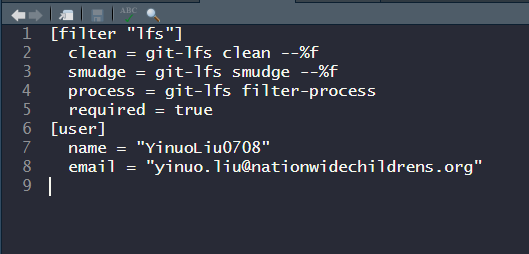
\includegraphics{images/Screenshot 2025-03-03 152728.png}

Enter your name and email address at line 7 and 8 and save the changes
(Ctrl + S).

Use the same user name and email address that you used to create your
Github account.

The code above {[}user{]} is to related to Git LFS (large file storage),
which is an extension of Git to help manage large files like datasets,
images, or videos. It's not necessary to establish git connection (only
your name and email are absolutely necessary).

If you find large file storage management important for your project,
feel free to copy and paste it into your .gitconfig file.

\begin{Shaded}
\begin{Highlighting}[]
\NormalTok{[filter }\StringTok{"lfs"}\NormalTok{]}
\NormalTok{  clean }\OtherTok{=}\NormalTok{ git}\SpecialCharTok{{-}}\NormalTok{lfs clean }\SpecialCharTok{{-}{-}}\NormalTok{ \%f}
\NormalTok{  smudge }\OtherTok{=}\NormalTok{ git}\SpecialCharTok{{-}}\NormalTok{lfs smudge }\SpecialCharTok{{-}{-}}\NormalTok{ \%f}
\NormalTok{  process }\OtherTok{=}\NormalTok{ git}\SpecialCharTok{{-}}\NormalTok{lfs filter}\SpecialCharTok{{-}}\NormalTok{process}
\NormalTok{  required }\OtherTok{=}\NormalTok{ true}
\end{Highlighting}
\end{Shaded}

Be mindful of space and symbols! Incorrect space and symbols may crush
the configuration. If you see error message related to .gitconfig,
reopen the file with the code edit\_git\_config() and check if
everything is correctly spelled and spaced.

\subsection{Step 3: Create a GitHub
token}\label{step-3-create-a-github-token}

A personal access token in GitHub is a secure, alphanumeric string that
grants access to your GitHub account and can be used instead of a
password for authentication.

Run the following code in console to create a personal access token.

\begin{Shaded}
\begin{Highlighting}[]
\NormalTok{usethis}\SpecialCharTok{::}\FunctionTok{create\_github\_token}\NormalTok{()}
\end{Highlighting}
\end{Shaded}

It will take you to a new webpage outside of RStudio that looks like
this:

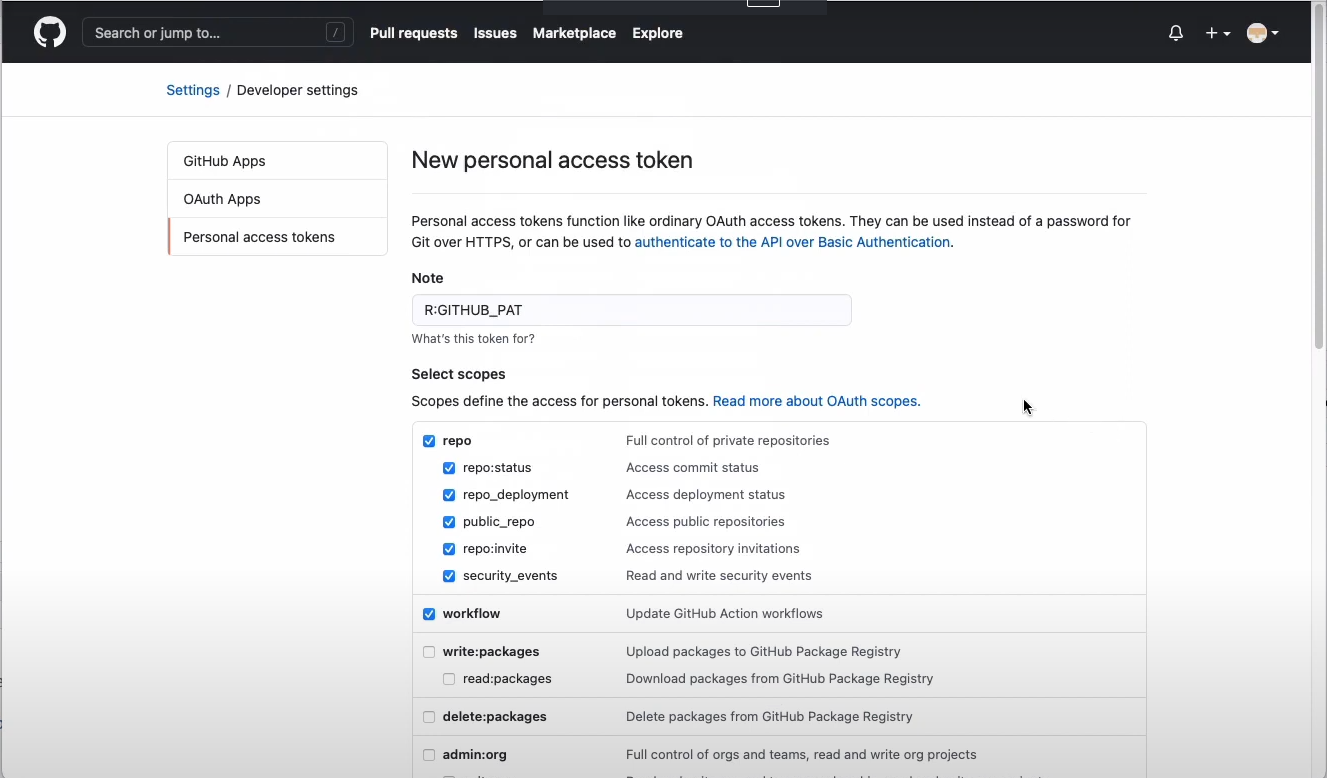
\includegraphics[width=8.90625in,height=\textheight]{images/Screenshot 2025-03-03 153024.png}

Give your personal access token a name (whatever you want!). Then scroll
to the bottom of the page and click `Generate new token'. It will take
you to a new page where you can copy your personal access token:

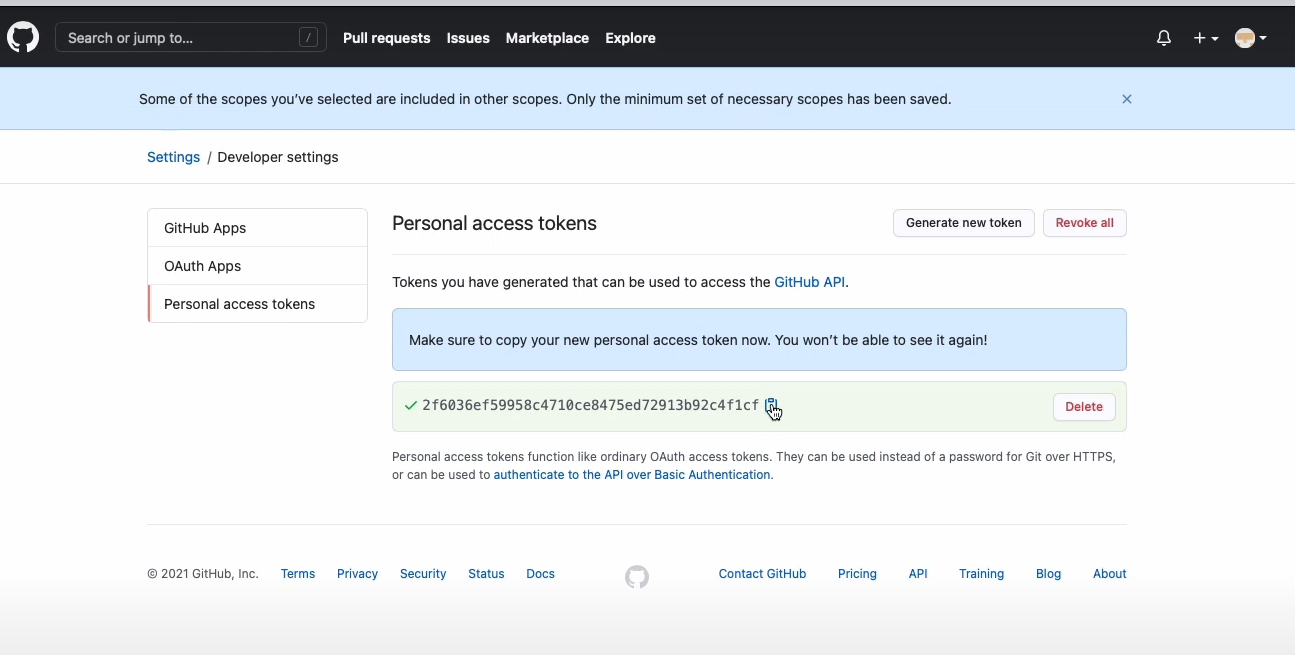
\includegraphics[width=8.89583in,height=\textheight]{images/Screenshot 2025-03-03 153127.png}

Copy your personal access token then go back to the console in Rstudio.
It is recommended to save a copy of the taken in a secure file in your
computer.

Typing the following code will open a dialog that asks you to enter your
token.

\begin{Shaded}
\begin{Highlighting}[]
\NormalTok{gitcreds}\SpecialCharTok{::}\FunctionTok{gitcreds\_set}\NormalTok{()}
\end{Highlighting}
\end{Shaded}

Enter you token.

You have configured RStudio to be linked to your GitHub account.

\subsection{Step 4: Create a local project and commit
changes}\label{step-4-create-a-local-project-and-commit-changes}

Now you can push your local project to GitHub and share it with your
team.

First, you can create a new project.

In the top left corner of RStudio, go to File -\textgreater{} New
Project, and you will see the following page

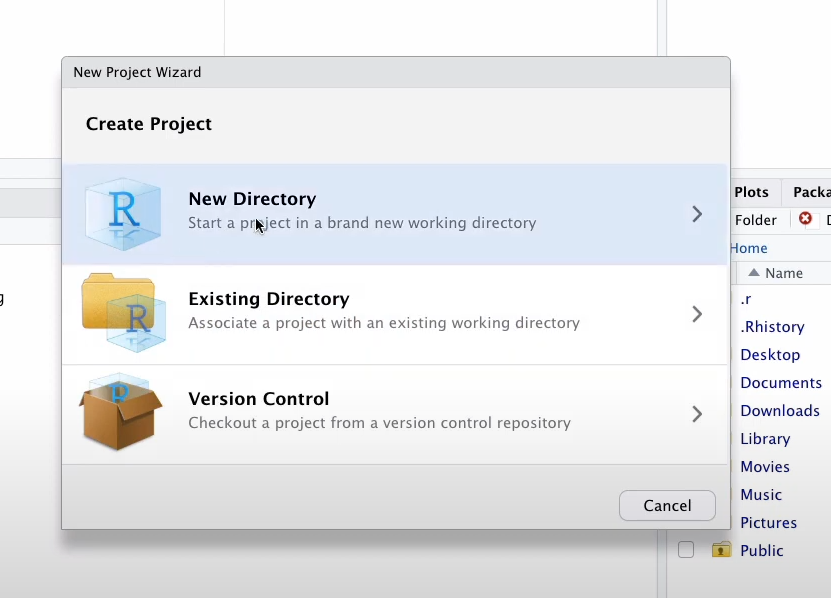
\includegraphics[width=5.9375in,height=\textheight]{images/Screenshot 2025-03-05 151204.png}

Click New Directory and choose a project type (Quarto for instance). It
will take you to this page:

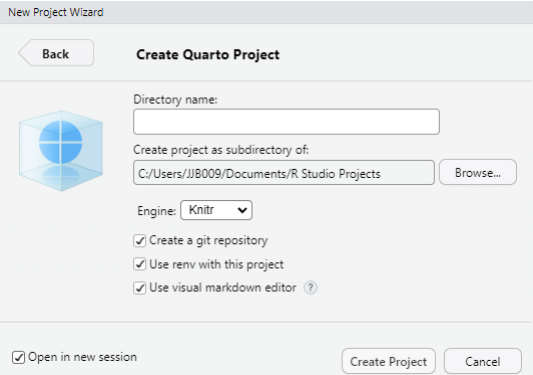
\includegraphics[width=5.91667in,height=\textheight]{images/Screenshot 2025-03-05 151400.png}

Give the project a name. Make sure you check all boxes. Then click
Create Project. Now you are in a new project!

To get connected with GitHub, run the following code in the console:

\begin{Shaded}
\begin{Highlighting}[]
\FunctionTok{library}\NormalTok{(usethis)}
\NormalTok{usethis}\SpecialCharTok{::}\FunctionTok{use\_git}\NormalTok{()}
\end{Highlighting}
\end{Shaded}

When RStudio asks you questions in the console, select yes for all
options (they may have it worded ``definitely'' or ``For sure'').

Now, you have initialized your new project as a Git repository.

Make sure that you have the Git tab in the top right section of R
studio.

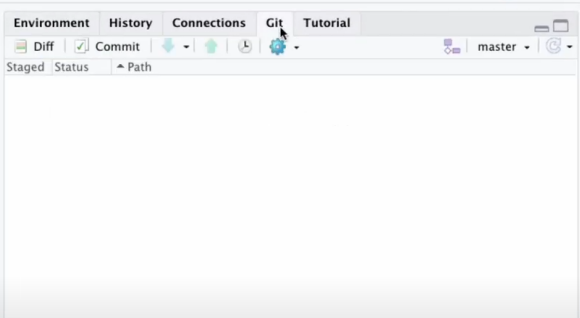
\includegraphics{images/Screenshot 2025-03-05 151716.png}

Create a new file in the project (could be R script, R markdown, or a
random file you like). Give the file a name and save it.

You can find that there is a file pop up in the right upper corner.

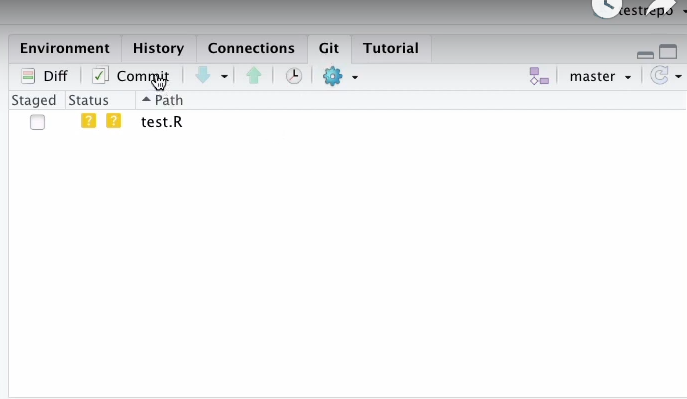
\includegraphics[width=6.61458in,height=\textheight]{images/Screenshot 2025-03-05 153220.png}

You need to commit the changes you made (adding a new file in this
case).

There are two ways to commit the changes: 1. type command in the
terminal, 2. use the Git window

\subsubsection{Commit method 1}\label{commit-method-1}

Go to terminal, type

\begin{Shaded}
\begin{Highlighting}[]
\NormalTok{git commit }\SpecialCharTok{{-}}\NormalTok{am }\StringTok{"describe the changes you made"}
\end{Highlighting}
\end{Shaded}

\subsubsection{Commit method 2}\label{commit-method-2}

Click Commit in the Git window, and you will see this page

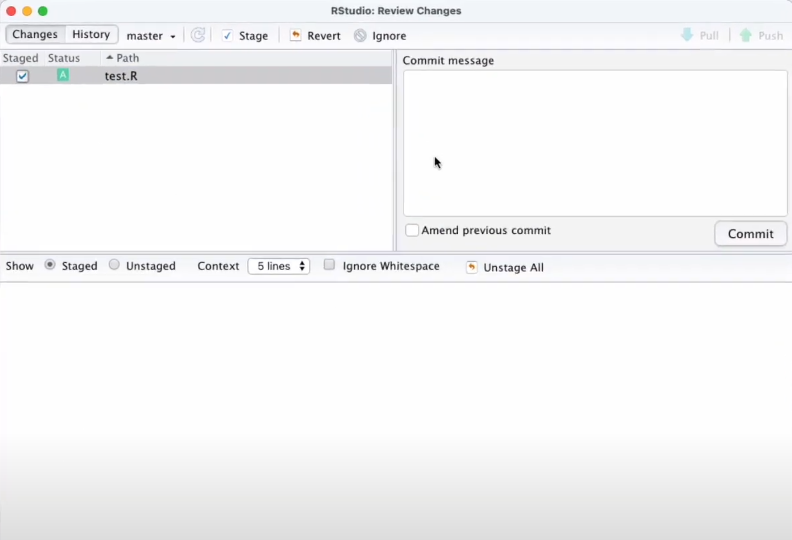
\includegraphics[width=7.04167in,height=\textheight]{images/Screenshot 2025-03-05 153653.png}

Remeber to check the staged box before the changes you want to commit.

Type in your commit message (you can't leave that box empty) and then
click Commit.

We recommend directly typing commands into the terminal to make commits,
as there is a variety of git commands that we will use in future team
collaboration. Don't let yourself be limited in the git window in
RStudio!

\subsection{Step 5: Push the local project to
GitHub}\label{step-5-push-the-local-project-to-github}

You have created a project and committed changes you made. The next step
is to push the local project to GitHub.

In console, type the code

\begin{Shaded}
\begin{Highlighting}[]
\FunctionTok{library}\NormalTok{(usethis)}
\FunctionTok{use\_github}\NormalTok{()}
\end{Highlighting}
\end{Shaded}

Now your project is pushed to GitHub!

Go to your GitHub page and find the corresponding project.

\subsection{Step 6: Pull from Remote
Repository}\label{step-6-pull-from-remote-repository}

In addition to push your local files to the remote end, you can also
pull stuff from the remote repository.

Type the following command in the terminal and hit Enter:

\begin{Shaded}
\begin{Highlighting}[]
\NormalTok{git pull}
\end{Highlighting}
\end{Shaded}

It will suggest that your files are ``Already up to date.''

Your local file has the same content as the remote repository, so
nothing more can be pulled and incorporated into your local files.

However, when you work with multiple team members in the future, always
remember to git pull before adding stuff, so you can keep up with all
the changes your teammates make.

Also remember to commit changes with accurate descriptions and push your
commits to the remote repository, so other members can keep track of
your work as well!

\subsection{Step 7: Creating Branches}\label{step-7-creating-branches}

\begin{tcolorbox}[enhanced jigsaw, breakable, opacityback=0, left=2mm, colback=white, arc=.35mm, toptitle=1mm, titlerule=0mm, opacitybacktitle=0.6, title=\textcolor{quarto-callout-tip-color}{\faLightbulb}\hspace{0.5em}{New concept alert!}, bottomtitle=1mm, rightrule=.15mm, toprule=.15mm, colframe=quarto-callout-tip-color-frame, bottomrule=.15mm, colbacktitle=quarto-callout-tip-color!10!white, leftrule=.75mm, coltitle=black]

You will learn an important feature of git -- branch in the next few
sections.

\end{tcolorbox}

The branching feature allows you to create independent lines of
development within a repository. This means you can work on new
features, experiments, or bug fixes without affecting the main codebase.

Type the following command to see all existing branches and the branch
you're at right now

\begin{Shaded}
\begin{Highlighting}[]
\NormalTok{git branch}
\end{Highlighting}
\end{Shaded}

There is only one master branch since you haven't created any new
branches yet. The master branch is marked as green to indicate that you
are here.

The master branch is the default branch in git repositories. People
often treat it as the stable version of your project, and changes are
merged into the master only after they've been thoroughly tested.

You may want to experiment with new code and features in your personal
branch instead of the master branch (which is a good practice of
coding). How to create a branch?

Here is the command:

\begin{Shaded}
\begin{Highlighting}[]
\NormalTok{git }\ControlFlowTok{switch}\NormalTok{ new}\SpecialCharTok{{-}}\NormalTok{branch}\SpecialCharTok{{-}}\NormalTok{name}
\end{Highlighting}
\end{Shaded}

Replace your preferred branch name in the command!

Try checking branches with this code

\begin{Shaded}
\begin{Highlighting}[]
\NormalTok{git branch}
\end{Highlighting}
\end{Shaded}

Now you will see two branches, one master, and one \textless whatever
you call your personal branch\textgreater, and the green mark suggests
that you are at the new branch you just created!

This is because the command - git switch branch-name - does two things
at the same time. It creates a new branch, and then switch your working
branch to the newly created one.

If you want to go back to the master branch, try

\begin{Shaded}
\begin{Highlighting}[]
\NormalTok{git }\ControlFlowTok{switch}\NormalTok{ master}
\end{Highlighting}
\end{Shaded}

Now you're back at the master! Great work creating new branches and
switching back and forth!

\subsection{Step 8: Merging Local
Branches}\label{step-8-merging-local-branches}

How do we synchronize the progress on different branches? The trick is
merge.

Let's first go back to the new branch you just created (command hint:
git switch branch-name). Add some new content like creating a new file,
writing down some random sentences. Save and commit these new changes
(command hint: git commit -am ``comments'').

Now switch back to the master branch. You will surprisingly find that
all the content you just added is not there. It's the purpose of
branches to keep work separate. It's also easy to synchronize the
progress on different branches with the following git command.

\begin{Shaded}
\begin{Highlighting}[]
\NormalTok{git merge name}\SpecialCharTok{{-}}\NormalTok{of}\SpecialCharTok{{-}}\NormalTok{branch}\SpecialCharTok{{-}}\NormalTok{you}\SpecialCharTok{{-}}\NormalTok{want}\SpecialCharTok{{-}}\NormalTok{to}\SpecialCharTok{{-}}\NormalTok{merge}
\end{Highlighting}
\end{Shaded}

Wait a few seconds, and you will see the newly added content shows up on
your master branch.

It's important that you stay or switch to the branch that you want new
changes be merged \textbf{into}, and specify the name of branch where
all changes come from in the git command.

Right now, you don't need to worry about the trouble of resolving merge
conflict, a condition that both branches affect the same line of code
which causes conflicts. When merge conflict shows up in the future (and
it will, frequently, in everyone's coding time), you will act as the
judge of branches and decide how to reconcile the differences.

\subsection{Step 8: Push Local Branches to Remote
Repository}\label{step-8-push-local-branches-to-remote-repository}

You want to publish your local branches in the remote repository, so
team members can see them.

You can push one specific local branch to the remote end with the
following command:

\begin{Shaded}
\begin{Highlighting}[]
\NormalTok{git push }\SpecialCharTok{{-}}\NormalTok{u origin branch}\SpecialCharTok{{-}}\NormalTok{name}
\end{Highlighting}
\end{Shaded}

You can also push all local branches to the remote end at once:

\begin{Shaded}
\begin{Highlighting}[]
\NormalTok{git push }\SpecialCharTok{{-}{-}}\NormalTok{all origin}
\end{Highlighting}
\end{Shaded}

It's a good practice to use different branches when working
collaboratively. It promotes isolation of work, which reduces the risk
of introducing bugs to the master branch. It facilitates parallel
development: multiple team members can work simultaneously on different
features. Though creating and interacting with branches may seem like a
burden to you right now, try embracing the idea of branches and
practicing it since it will make your future work easier.

\subsection{Step 9: Create Pull Request on
GitHub}\label{step-9-create-pull-request-on-github}

Add something new on your local branch other than the master branch, add
and commit the changes (command hint: git commit -am ``comments''), then
push to this local branch to the remote repository (command hint: git
push -u origin branch-name).

After the changes on your local branch is committed and pushed, navigate
to the GitHub page. You will see a notification like this.

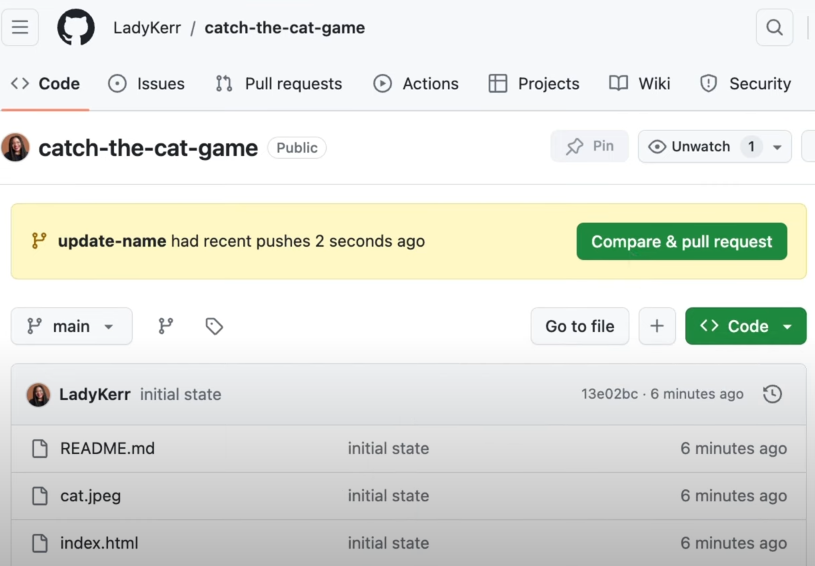
\includegraphics[width=6.29167in,height=\textheight]{images/Screenshot 2025-03-20 152935.png}

This notification occurs because your feature branch is ahead of your
master branch, meaning that the feature branch has changes not in the
master branch. GitHub captures this discrepancy in branches, and it
wants to make sure that the master branch is up-to-date, so it suggests
to make a pull request to update the master branch.

If you feel good about merging new changes to the master branch, click
Compare \& pull request.

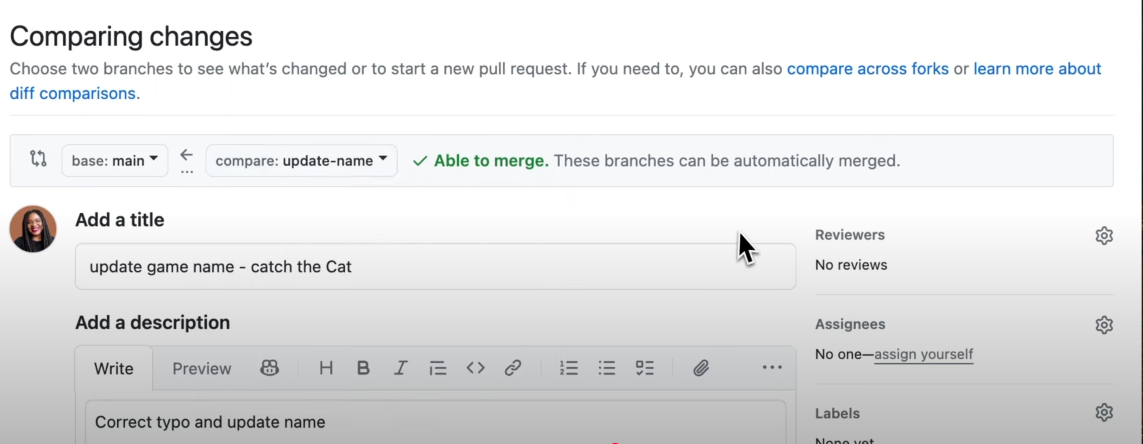
\includegraphics{images/Screenshot 2025-03-20 153625.png}

You will see a page like that. Pay attention to the header. The base
branch is the branch all the new changes will be merged into, and the
compare branch is where the changes come from. The green words Able to
merge indicates that there is no conflict between these two branches,
and you can easily merge the branches.

Add a title and a description to this pull request if you want to, then
scroll down and click Create pull request.

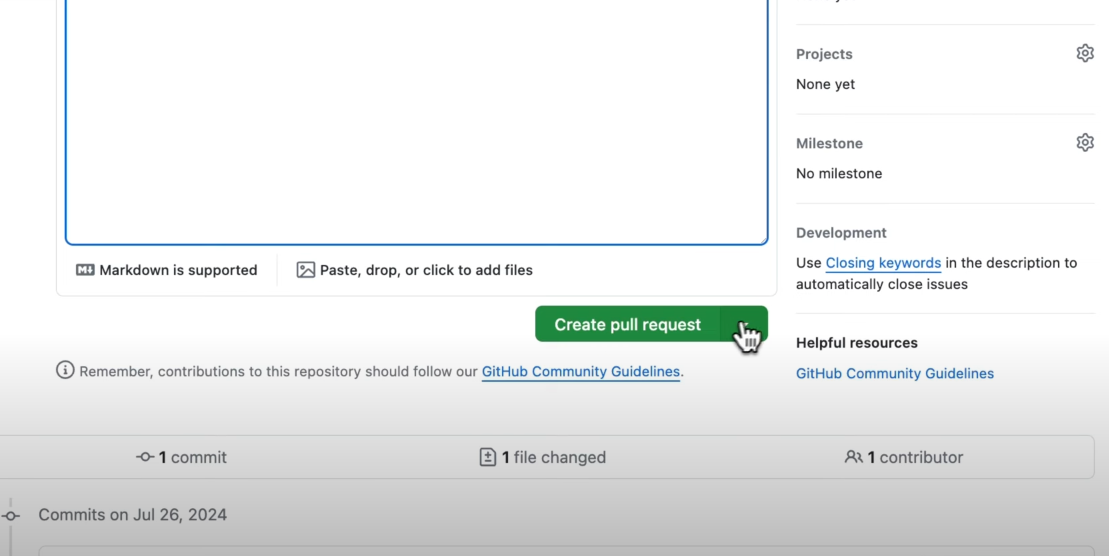
\includegraphics{images/Screenshot 2025-03-20 154007.png}

You just created your first pull request! Navigate back to the code
page, check out the master branch, and you will find that the edits you
made on the feature branch are there on the master branch.

If you are working with multiple team members, remember to consult other
members' opinions before creating and executing pull requests. You don't
want to change the base code that everyone will work on before notifying
other people.

\subsection{Step 10: Clone Git Repository in
RStudio}\label{step-10-clone-git-repository-in-rstudio}

Now you have some basic knowledge of Git, GitHub, and branches. It's a
good time to really interact with a shared project that multiple people
work on. You first need to obtain a copy of the project.

Cloning a Git repository in RStudio allows you to create a local copy of
a project from GitHub.

First, you need to access the GitHub repository you want to clone.

Take this toy project for example. You will see this page

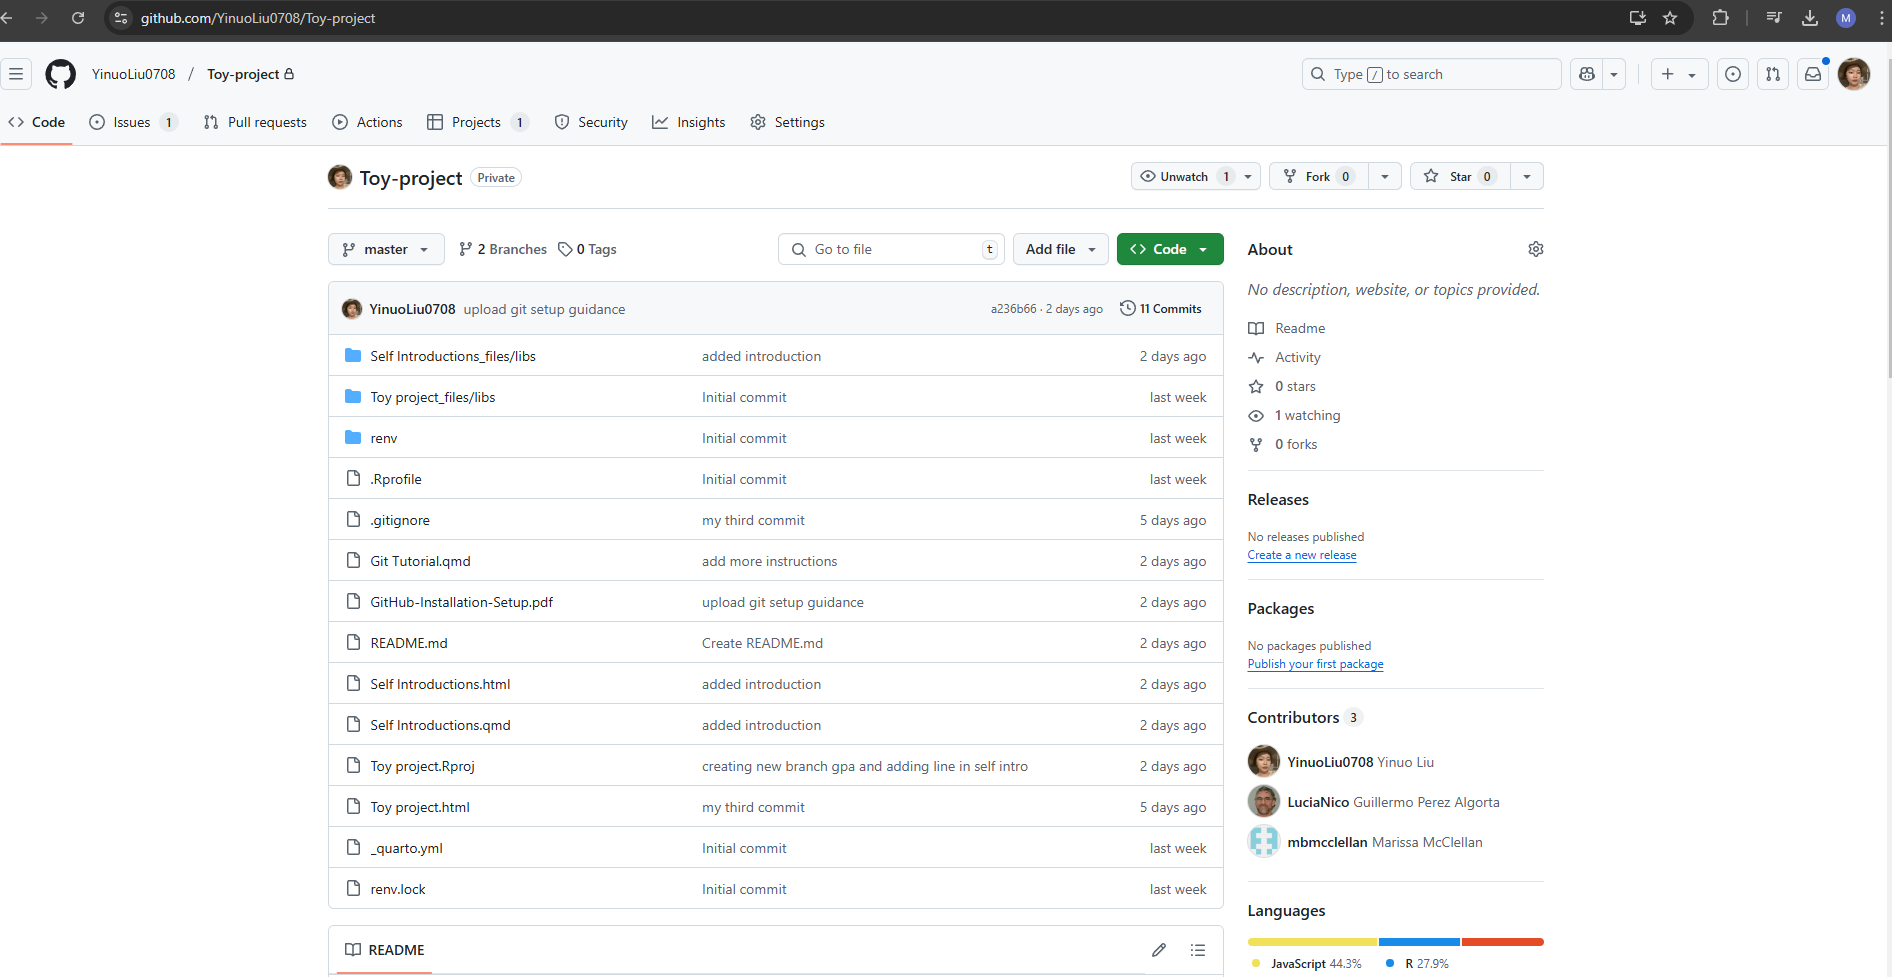
\includegraphics[width=9.04167in,height=\textheight]{images/Screenshot 2025-03-05 155840.png}

Click on the green Code button. Then, copy the http URL to the
clipboard.

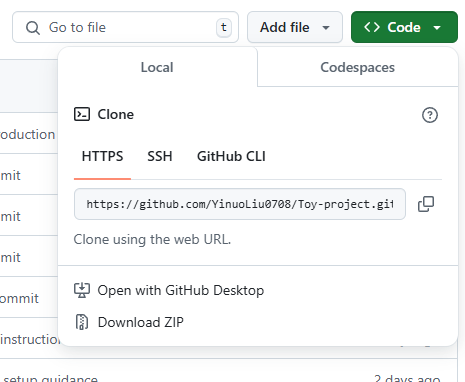
\includegraphics[width=5.73958in,height=\textheight]{images/Screenshot 2025-03-05 160008.png}

Open a new session in RStudio (Go to Session -\textgreater{} New
Session).

In the top left corner of RStudio, go to File -\textgreater{} New
Project, then choose Version Control.

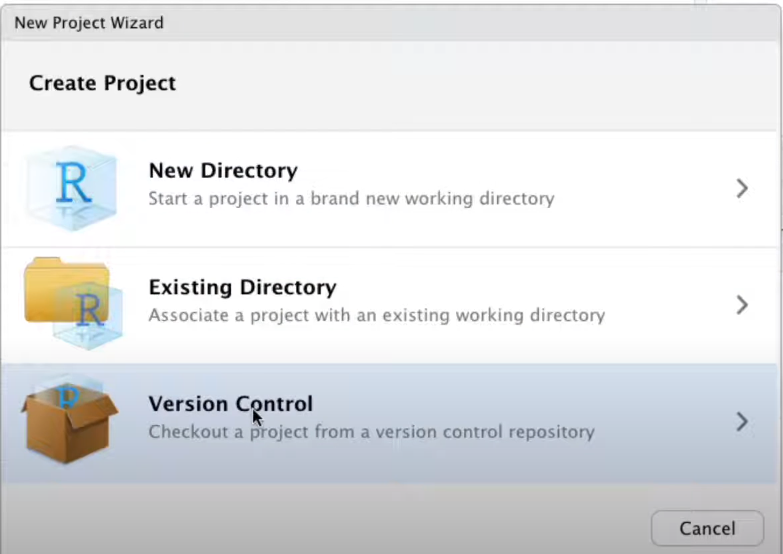
\includegraphics[width=5.92708in,height=\textheight]{images/Screenshot 2025-03-05 160414.png}

That will open a new window with two options, choose Git

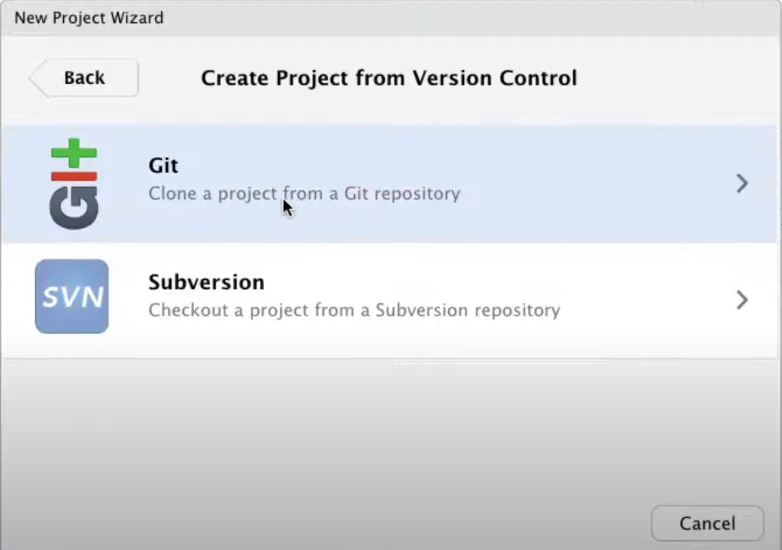
\includegraphics[width=5.91667in,height=\textheight]{images/Screenshot 2025-03-05 160503.png}

Now, paste the link you copied from GitHub into Repository URL. Then
click Create Project.

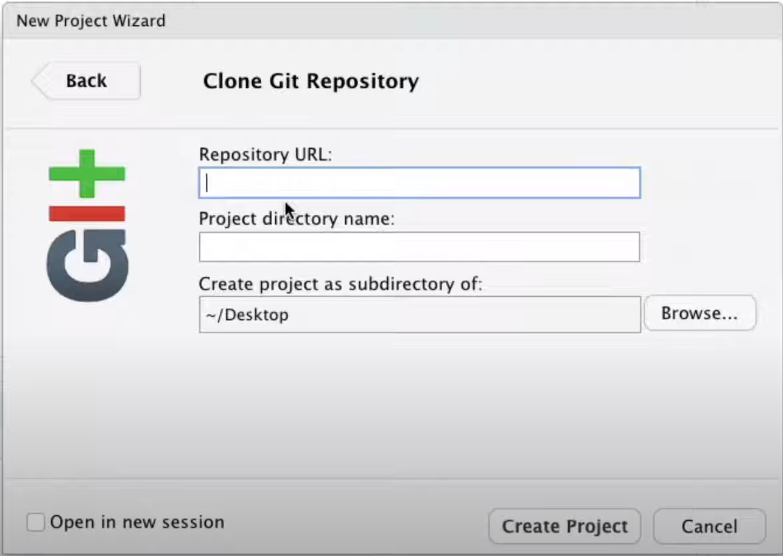
\includegraphics[width=5.98958in,height=\textheight]{images/Screenshot 2025-03-05 160543.png}

You have a copy of the Toy project from the remote depository on GitHub!

\subsection{Step 11: Practice!}\label{step-11-practice}

It's a good time to practice all the commands you learned in this
tutorial.

Try the following tasks

\begin{enumerate}
\def\labelenumi{\arabic{enumi}.}
\tightlist
\item
  create a branch named as your preferred name
\item
  add your introduction in Self Introductions.qmd
\item
  Commit all the changes you made
\item
  Push the local branch to the remote end
\end{enumerate}




\end{document}
